\documentclass[12pt]{article}
% This first part of the file is called the PREAMBLE. It includes
% customizations and command definitions. The preamble is everything
% between \documentclass and \begin{document}.

\usepackage[margin=1in]{geometry}  % set the margins to 1in on all sides
\usepackage{graphicx}              % to include figures
\usepackage{amsmath}               % great math stuff
\usepackage{amsfonts}              % for blackboard bold, etc
\usepackage{amsthm}                % better theorem environments

\usepackage{rotating} % for sideway table
\usepackage{xcolor}
\usepackage{hyperref}
\hypersetup{
    colorlinks,
    linkcolor={red!50!black},
    citecolor={blue!50!black},
    urlcolor={blue!80!black}
}
\usepackage{cleveref}

\usepackage{array,tabularx}

\newenvironment{conditions*}
  {\par\vspace{\abovedisplayskip}\noindent
   \tabularx{\columnwidth}{>{$}l<{$} @{${}={}$} >{\raggedright\arraybackslash}X}}
  {\endtabularx\par\vspace{\belowdisplayskip}}
  
\usepackage{float}
\restylefloat{table}

% various theorems, numbered by section

\newtheorem{thm}{Theorem}[section]
\newtheorem{lem}[thm]{Lemma}
\newtheorem{prop}[thm]{Proposition}
\newtheorem{cor}[thm]{Corollary}
\newtheorem{conj}[thm]{Conjecture}

\DeclareMathOperator{\id}{id}

\newcommand{\bd}[1]{\mathbf{#1}}  % for bolding symbols
\newcommand{\RR}{\mathbb{R}}      % for Real numbers
\newcommand{\ZZ}{\mathbb{Z}}      % for Integers
\newcommand{\col}[1]{\left[\begin{matrix} #1 \end{matrix} \right]}
\newcommand{\comb}[2]{\binom{#1^2 + #2^2}{#1+#2}}

% bibliography
\usepackage{natbib}
\bibpunct{(}{)}{;}{a}{}{,} % no comma between author and year

\title{Prospectus: FDI, corruption, and the effect on private sector development}
\author{Anh Le}


\begin{document}
\maketitle

\section{Empirical Puzzle}
In recent decades, foreign direct investment (FDI) global flow has steadily increased, rising to over \$1.5 trillion dollars in 2014. For developing countries, FDI flow is also remarkably robust to global downturn, leading to enthusiastic endorsement by major international organizations as a key factor to economic development (\Cref{fig:globalfdi}).\footnote{http://www.imf.org/external/pubs/ft/fandd/1999/03/mallampa.htm, http://www.weforum.org/reports/foreign-direct-investment-key-driver-trade-growth-and-prosperity-case-multilateral-agreement} This assumption is also shared widely within political science, where much of the literature starts with the assumption that countries want to seek FDI for its many benefits. The question that these works focus on is \textit{how} countries can attract FDI, not \textit{whether} they want to do so \citep{Jensen2003, Li2003, Li2006, Ahlquist2006}.\footnote{Two recent exceptions are \citet{Pinto2013, Pandya2013}, which are the first to investigate the demand for FDI.} 

\begin{figure}[!ht]
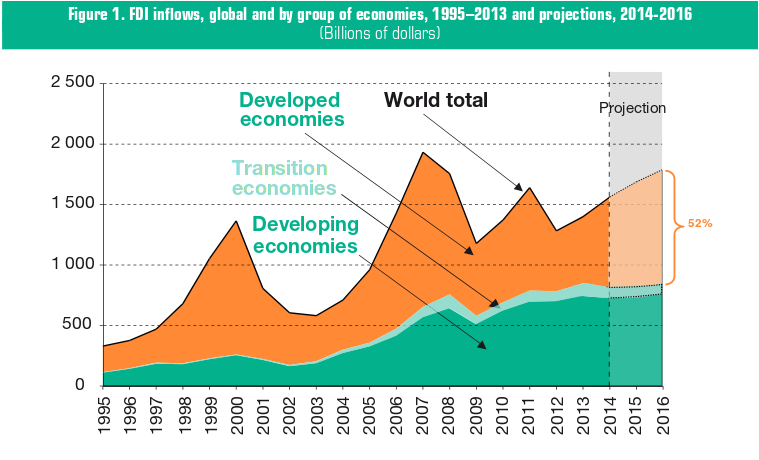
\includegraphics[width=\textwidth, height=\textheight,keepaspectratio]{../figure/global_fdi}
\caption{Source: World Investment Report, 2014}
\label{fig:globalfdi}
\end{figure}

Underlying this mode of thinking is the assumption that FDI brings various benefits to developing countries, including capital and employment. However, the most important promise that FDI holds to growth is the spillover of productivity between foreign firms and domestic firms. This can happen if local firms hire workers that were trained in a foreign firms, improve productivity through backward and forward linkages, or imitate foreign technology. According to growth theory, it is FDI's spillover, not capital or employment, that brings the technological innovation that is requisite for economic growth \citep{Findlay1978}. In this view, FDI is also a public good, providing spillover benefits to the local firms in ways that foreign firms do not take into account in their private calculations. This provides the justification for countries' using investment incentives to rectify the undersupply of FDI, closing the gap between private and social returns. 

Despite this prevailing view, there is little conclusive evidence of FDI having a positive effect on growth \citep{Nair-Reichert2001, Carkovic2002} or poverty reduction \citep{Guerra2009} (\Cref{fig:fdipoverty}). A substantial literature has developed to explain this puzzle, concluding that the growth-enhancing and spillover effect of FDI is conditional on the absorptive capacity of local firms. Cross-nationally, scholars find that FDI is more likely to have a positive growth effect when the technological gap between the local and foreign firms are small \citep{Nunnenkamp2004} and when host countries have strong financial and institutional development \citep{ Durham2004}. Similarly, absorptive capacity, measured by the level of schooling in host economy, conditions the transfer of technology between foreign and local firms across regions in China \citep{Fu2008} and countries in Latin America \citep{Willem2004}.

\begin{figure}[!ht]
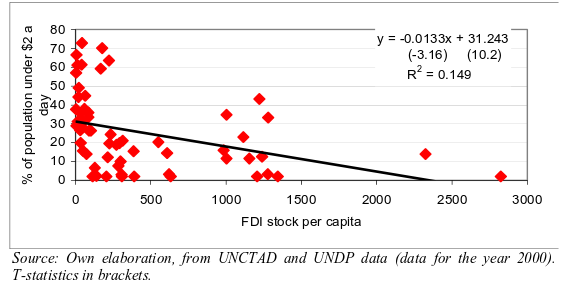
\includegraphics[width=\textwidth, height=\textheight,keepaspectratio]{../figure/fdi_poverty}
\caption{Relationship between FDI and poverty}
\label{fig:fdipoverty}
\end{figure}

Despite the resounding conclusion that the effect of FDI is highly conditional and that investment incentives do not work, why do countries still fixate so much on bringing in FDI instead of developing local absorptive capacity \citep{Blomstrom2002}? For example, Ireland provided foreign investors with lower tax rate, lower land price, and cash grants for R\&D that do not need to be repaid. China also used a tax holiday (two years of no tax and three year of half the normal tax rate) in special economic zones to attract more foreign firms \citep{Telford2001}. We see the same widespread use of investment incentives in Southeast Asia \citep{Fletcher2002}. In Vietnam, the race to offer incentives to foreign firms rages on even among sub-national units, as provincial governments defied the central government's directive and offered extra-legal incentives to FDI firms \citep{Vu2007}. Not only do these measures not work in attracting more FDI, they also deprive countries of revenues that could be spent on improving the local labor quality and investment climate, which are much more conducive to spillover effect and growth.

Thus, my dissertation project focuses on this empirical puzzle: if the positive effect of FDI is uncertain, why is there so much focus on attracting it? If developing absorptive capacity is so crucial to making FDI growth-enhancing, why is it often neglected? To understand this puzzle, I propose that we need to take into account the calculus of the individual bureaucrats and government officials, who may be more interested in the potential rents from foreign firms than the spillover and growth-enhancing effect of FDI. This is a potential reason why we often see countries (i.e. government officials) being so enthusiastic about attracting FDI, yet not so passionate about developing the local capacity that enables FDI to actually have a positive effect on growth.

\begin{figure}[!ht]
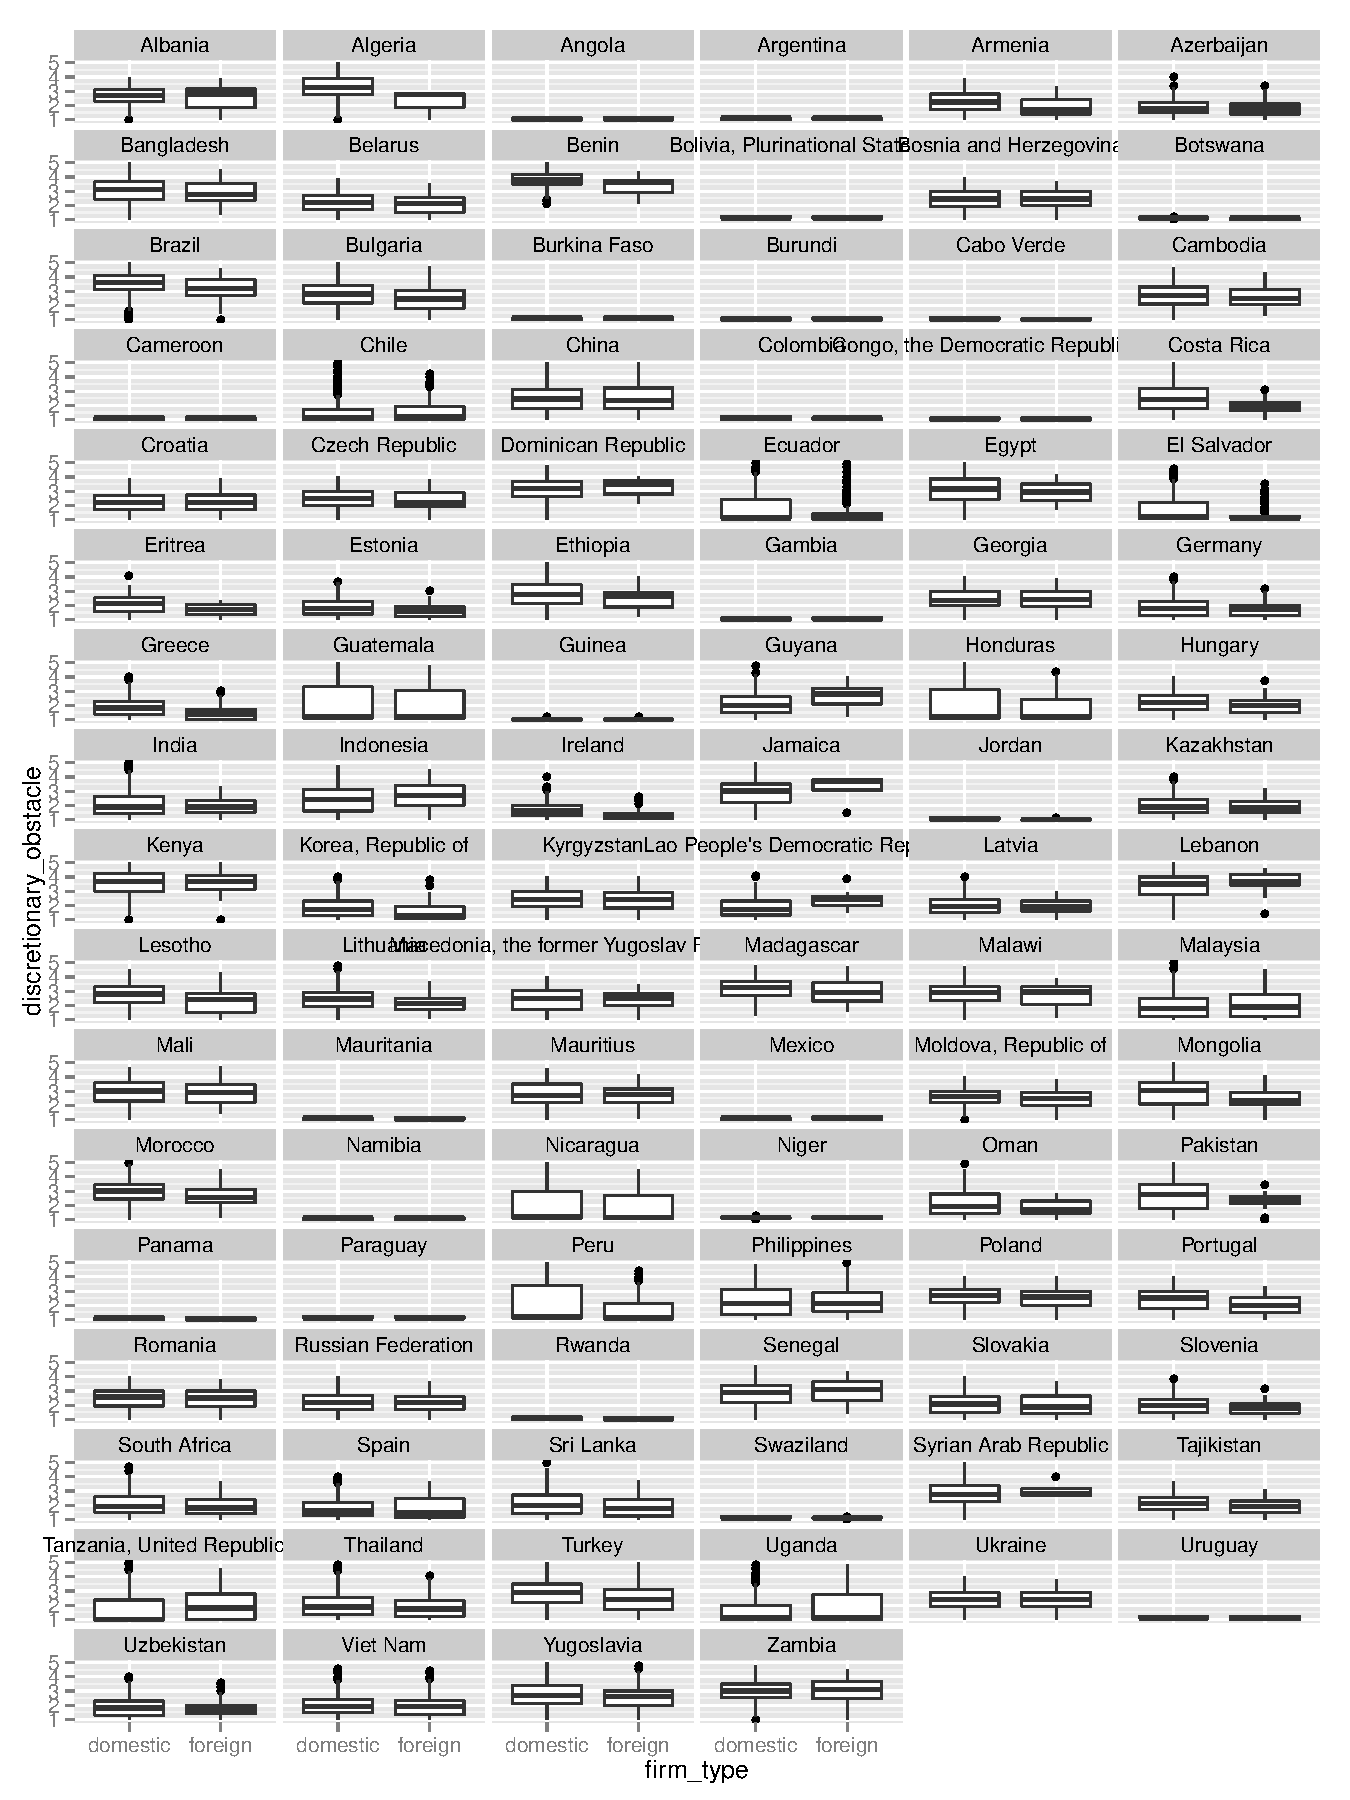
\includegraphics[width=\textwidth, height=\textheight,keepaspectratio]{../figure/fdi_domestic_treatment}
\caption{The treatment of FDI and domestic firms across countries}
\label{fig:fdi_domestic_treatment}
\end{figure}

Starting with this empirical puzzle, my project also sheds light on various related issues. First, it investigates the collusion of FDI firms and host countries' officials, a understudied phenomenon as the existing literature often assumes a foreign firm trying to fend off extortion and harassment from host countries. Second, it examines the political drivers behind private sector development, an issue whose welfare impact is well-known yet whose political determinants are ill-understood. Third, my project looks at the treatment of foreign firms versus domestic firms from a fresh angle. The majority of political science literature has considered FDI the underdog, unfamiliar with the location, susceptible to expropriation, and threatened by the lobbying effort of domestic firms. However, when FDI firms are big and resourceful, they can be an equal partner in the collusive relationship with corrupt officials to the detriment of the domestic sector.


\section{Tentative evidence}
In this section, I present some evidences that motivate the puzzle.

\begin{itemize}
	\item The spillover effect of FDI on growth is highly variable. For example, FDI is found to be growth-enhancing in East Asia, but not in Latin America \citep{Zhang2001}. Similarly, the effect of FDI on domestic investment also varies across countries and regions. FDI is found to crowd in investment in some countries (e.g. Ghana, Senegal, South Korea, Pakistan, Thailand, etc.) but crowd out in others \citep{Agosin2005}.
	
	\item Despite the prevalent concern with discrimination against foreign firms, the Wold Bank Enterprise Survey finds that foreign firms actually face fewer obstacles while doing business \citep{Batra2003}. The gap in the treatment of foreign and domestic firms also varies across countries (\Cref{fig:fdi_domestic_treatment}).
	
	\item The correlation between corruption and FDI is negative. However, there is a lot of unexplained variance at the high end of FDI. Countries with low level of FDI are always very corrupt, but countries with high level of FDI can be as well (\Cref{fig:fdi_corruption}).
	
	\begin{figure}[!ht]
	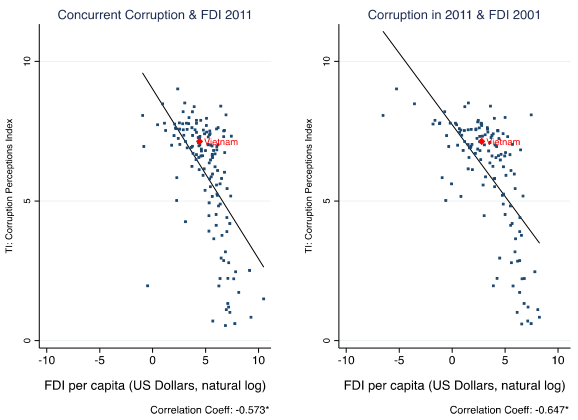
\includegraphics[width=\textwidth, height=\textheight,keepaspectratio]{../figure/fdi_corruption}
	\caption{Source: \citep{Malesky2015}}
	\label{fig:fdi_corruption}
	\end{figure}
\end{itemize}


\section{Theory}
\subsection{``Price of spillover'' sectoral variation}

As implied in the theory section, when the ``price'' of spillover is high (i.e. it is difficult to obtain spillover given the country's absorptive capacity or sector-specific characteristics), the government official would choose a bundle that has more private benefit than spillover. 

PICTURE

Here I focus on industry-specific characteristics that either facilitate or hinder spillover. Due to its divisible process, manufacturing firms tend to engage more local suppliers and generate more spillover effect than primary and tertiary sectors. In addition, there is a wide variation across industries within a sector to be exploited as well. For example, in manufacturing, food processing can have a high amount of spillover due the sourcing of raw materials and packaging, whereas in textile and automotive industries (which require high level of technological sophistication), it is harder for foreign firms to work with local suppliers. Similarly, in tertiary sectors, finance, trading, tourisms and utilities are is generally not divisible into discrete stages to subcontract. Yet service industries such as retailing and construction have more opportunities for input suppliers (cite).

This leads us to the following hypothesis:

\begin{quote}
Hypothesis: Government official will pursue less private benefits from firms in industries where it is easier to generate spillover
\end{quote}

While such variation across industry is clear conceptually, measurement is thorny given the many factors that can affect the potential for spillover. In addition, there is an endogeneity problem as the potential for spillover may itself be affected by the level of rent-seeking of that industry. For example, an industry plagued by collusive relationship between the official and the foreign firms does not offer an enabling environment that allows private firms to develop their absorptive capacity. The endogeneity problem is compounded if the official strategically invests to improve absorptive capacity, in which case it is not even clear which direction is our estimate biased.

To address both of these measurement and endogeneity issues, I will use the variation in technological spillover across industries in the United States as the instrumental variable.\footnote{The United States is considered due to its high quality economic data. Alternatively, for each country, I can use a comparable country in the same region or the same developmental stage to formulate the instrument} The assumption is that the level of technological spillover in a US industry only correlates with the level of bribe in another country's industry through the latent factor that is the industry-specific potential for spillover.

\subsection{``Price of private benefit'' firms ability to bribe}

As implied from the theory, when the ``price'' of private benefit is high (i.e. it is costly for the firm to offer the official private benefit), the official would choose a bundle that has less private benefit.

This theoretical claim generates many substantive predictions that we can test, each involving a factor that affect the cost of bribing for firms. For example, foreign firms that come from a corrupt home countries may have more experience with bribing and thus would incur less information cost if they bribe.

Here I focus on the Phase 3 (Enforcement) of the OECD Anti-Bribery Convention (ABC) as an exogenous increase in the cost of bribing for foreign firms in Vietnam. In December 1997, all members of OECD and an additional five non-members, accounting for nearly 61\% of world trade, signed the ABC. The ABC criminalizes the bribery of foreign public officials and upholds its principles with a peer-monitoring system, in which member countries visit and review one another's legislation and implementation. According to legal experts, these reports are often quite harsh and effective in shaming countries into improving their practices \citep{Tyler2011}.

Important for my research design, in December 2009 the OECD's Working Group on Bribery (WGB) annouced that following Phase 1 and 2 (Evaluation and Assessment) there would be a Phase 3 (Enforcement). The goal of Phase 3 is to continually monitor countries' anti-bribery practices and to exhort inactive enforcers. Noticeably, Phase 3 also removed a previous exception that allowed firms to make ``small facilitation payment'' \citep{Strauss2013}. Researchers have argued that following the announcement of Phase 3, member countries ramped up enforcement to avoid a negative review, and causing their firms to reduce bribery abroad \citep{Malesky2015b}. 

Given that FDI to Vietnam only accounts for a small fraction of OECD countries' total foreign investment, it is plausible that Vietnam is not a major factor driving the initiation of Phase 3. Therefore, the announcement of Phase 3 serves as an exogenous shock to the cost of bribery for firms from ABC member countries. With OECD firms being reluctant to offer bribes, we expect corrupt officials to become uninterested in OECD firms. Post 2009, OECD firms would be attractive only to non-corrupt officials for their developmental impact, and we should observe them having more spillover effect.\footnote{An alternative design looks at the difference between OECD and non-OECD firms that \textit{enter} Vietnam pre- and post-2009. This design will have fewer firms in the sample but could be more appropriate if we think that the spillover-bribe bundle is negotiated at the time firms enter Vietnam and is hard to change later, even with the ABC coming into effect. If so, the change in level of spillover and bribe is caused by the change in the official's selection of firms instead of the adjustment in behaviors of existing firms after 2009.}

With 2009 as an exogenous shock we have a difference-in-difference design. First, we estimate the difference in spillover between OECD and non-OECD firms, pre-2009. We then find the same difference in spillover post-2009. Subtracting these two differences, we can estimate the effect of corruption on the level of spillover.

I sum, I have the following hypothesis:

\begin{quote}
Hypothesis: The Phase 3 (Enforcement) of OECD's Anti-Bribery Convention causes firms from member countries to have more spillover and pay less bribe.
\end{quote}


\subsection{Time horizon of officials}

As implied by the theory above, an official with a longer time horizon would choose a bundle with more spillover, whereas an official with a short time horizon would choose a bundle with more private benefit.

To get a handle on the time horizon of the official, we need to know the options provided to the official within the country's political economic system. Such is a big and difficult question to study with a cross-national design due to an insurmountable degree of endogeneity stemming from unobservable and unmeasurable differences across political systems. Therefore, at this step, I focus on the case of Vietnam, whose sub-national variation in FDI flow and private sector development serve as an excellent testing ground. Again, here I focus on bribe and informal fees as the main form of private benefit for officials. Such constraint is not problematic for the case of Vietnam, where the authoritarian system means that officials are not offered campaign contribution and where revolving door jobs are non-existent.

\subsubsection{The effect of time horizon on the choice of Vietnamese provincial officials} 

The relative weight assigned to spillover versus bribe by the Vietnamese provincial officials is determined by the principal-agent relationship between Vietnam's central and the provincial governments. On the one hand, the central government (i.e. the principal) cares more about the spillover effect of FDI and uses promotion to reward local officials that attract high-spillover FDI. On the other hand, local officials (i.e. the agent) have more opportunities to engage in corruption with foreign firms, and should they decide that the private benefit of corruption is greater than that of promotion, they will prioritize foreign firms that bring bribes over those that have high spillover effects.

The reason behind such difference in the preference of central and local governments is the fact that FDI projects are approved and managed at the provincial level. While the central law may be uniform in the book, its implementation varies widely across sub-national units in Vietnam \citep{Meyer2005}.\footnote{Vietnam's sub-national variation in implementation generalizes well to other cases, such as China \citep{Thun2006}} Therefore, the provincial government holds valuable services for sale to foreign firms. In contrast, the central government is more removed from direct contact with FDI firms and thus less likely to benefit from corruption than provincial leaders. 

In addition, the central government is much more concerned with overall economic growth, which is central to the longevity of the regime \citep{Malesky2008}. It wants to attract high-spillover FDI and uses promotion to reward local officials that accomplish this goal. On the other hand, each provincial leader is incentivized to free-ride on the developmental effort of other provinces and of the central to keep the entire regime stable. Therefore, local officials value the spillover effect of FDI only insofar as the opportunities for promotion that it brings.

Fortunately for the central government, the principal-agent problem in this context is partially solved because monitoring is not too difficult. Indeed, the central government can observe the economic performance of the provinces and use personnel management to punish and reward provincial officials \citep{Sheng2007, Li2005}.\footnote{\citet{Shih2012} recently argue that economic performance does not matter to cadre promotion. However, they investigate all members of the Chinese Central Committee, including the central party apparatus, the army, and the central economic bureaucracy. These actors are not the important decision-makers in our theory.} Therefore, the principal-agent problem is only severe when provincial officials are not interested in further promotion to the central government, i.e. when the local official's time horizon is short. This suggests that there will be a variation in the level of FDI's spillover effect across provinces according to provincial officials' interest in promotion. In the research design, I use fuzzy regression discontinuity (RD) exploiting the mandated retirement age of Vietnamese officials, arguing that those that are in their last term have shorter time horizon and less interest in promotion. 

By looking at this variation in the career interest of provincial officials, my theory contributes a fresh angle to the current literature on the relationship between decentralization and corruption. So far, scholars have only postulated a one-way relationship: either decentralization increases bribery \citep{Fan2009} or reduces it \citep{Guerra2009}. In my model, how decentralization affects corruption is conditional on the local officials' interest in the promotions offered by the central as carrots.


Three key assumptions in the theory above deserve further examination:
\begin{enumerate}
\item Why wouldn't Vietnam's central government worry that a developed private sector may lead to social change that ultimately undermines its rule?

First, there is a large scholarship showing that authoritarian regimes are very adept at using institutions to manage regime outsiders in general and business in particular \citep{Gandhi2006, Gandhi2008, Wright2008, Le2015}. Second, if the legitimacy of the regime rests heavily on delivering economic growth, then the short-term risk of an economic downturn creating instability features much more prominently than the long-term concern with social changes. Third, it is possible to foster economic growth while restricting political freedom (e.g. Singapore). Indeed, growth can make a regime, both democratic and authoritarian, more stable, and creates room for political control \citep{Przeworski1997}.

\item Why don't provincial leaders seek rent from the domestic sector? 

First, Vietnam's private sector was very small when FDI was first allowed into Vietnam. The size and the profitability of the average domestic firm is still smaller than those of foreign firms today. Therefore, there are both fewer rents and more coordination problems if provincial officials want to seek rents from domestic firms. Second, ironically, if officials want to grow the private sector for future rent-seeking, they must promote an enabling business environment that are free from rent-seeking. In contrast, engaging in corruption with large and existing FDI firms is much more convenient. Essentially, corrupt provincial officials have shifted the cost of building a thriving domestic sectors to the home countries of FDI firms and now extract rents from the high productivity and high profitability of these firms. 
\end{enumerate}

In sum, I propose a hypothesis about variation across Vietnam's provinces:

\begin{quote}
Hypothesis: In provinces whose leaders are in their last term before the mandated retirement age, there are more spillover and less bribe from the foreign firms.
\end{quote}



\section{Research design}
\subsection{Measuring the main dependent variable: spillover effect}
\label{sec:measure_spillover}

\subsubsection*{Measuring spillover indirectly}

Similar to how growth economists start endogenizing technological change, FDI researchers investigate how technology spillover from FDI may happen instead of assuming its inevitability \citep{Romer1994}. Several channels for spillovers have been proposed, some of which suggest an indirect measure of technology spillover.

These channels are:
\begin{itemize}
	\item imitation:  private firms may reverse engineer a production or management technique \citep{Wang1992}, which is facilitated by backward linkage between local and foreign firms \citep{Javorcik2004}. This motivates my first measure of spillover effect: \% of private firms that participate in contracts with foreign firms.
	\item competition: similar to the effect of competition from arm's length trade on productivity, the presence of foreign firms in the domestic market put pressure on local firms to reduce inefficiency \citep{Glass2002}.
	\item export demonstration: foreign firms are more knowledgeable about exporting, which involves high fixed cost to set up a distribution and transport infrastructure, or learning about foreign taste and regulatory environment. Domestic firms can learn this ``export know-how'' from foreign firms \citep{Aitken1997}. This motivates my third measure of spillover effect: \% of private firms that export.
	\item skills acquisition: workers trained in foreign firms bring along their human capital when they move to domestic firms \citep{Djankov2000}. This presumes a healthy domestic sector that can offer competitive wages to workers.
\end{itemize}

Among these channels, \textit{imitation} and \textit{export demonstration} forms the theoretical basis of my two proxy measurements of spillover:
\begin{enumerate}
\item frequent business contacts between foreign and domestic firms,
\item percentage of domestic firms engaging in export
\end{enumerate}

\subsubsection*{Measuring spillover directly}

As standard in the economic literature that studies whether there is a spillover effect for FDI, we can also measure spillover directly. This is done in two steps \citep{VanBeveren2012}.

\begin{itemize}
\item First, measure the level of technology or productivity of a firm.

Level of technology: R\&D spending

Level of productivity: Consider the familiar Cobb-Douglas production function:

\begin{align}
Y &= AL^{\alpha}K^{\beta}
\end{align}

where $Y$ is value added, $A$ is total-factor productivity (TFP), $L$ is labor, and $K$ is capital. $y$, $L$, and $K$ are observable, while $A$ is not. Log transform both sides of the equation, we attain a linear form:

\begin{align} \label{eq:cobb_douglas_linear}
y &= a + \alpha l + \beta k
\end{align}

where the lowercase variables are the log-form of the uppercase variables (e.g. $y = \log(Y)$ and so on). \autoref{eq:cobb_douglas_linear} can then be estimated with OLS:

\begin{align} \label{eq:cobb_douglas_OLS}
y_i = \beta_0 + \beta_1 l_i + \beta_2 k_i + \epsilon_i
\end{align} 

where $\beta_0$ is the average total-factor productivity of all firms and $\epsilon$ is the firm-specific deviation from that mean. From the estimated coefficients of \autoref{eq:cobb_douglas_OLS}, we can estimate firm-level TFP as follows:

\begin{align}
a_i &= \hat\beta_0 + \hat\epsilon_i \\
A &= \exp^{\hat\beta_0 + \hat\epsilon_i}
\end{align}

\item Having estimated firm-level TFP (or technology), we then regress TFP (or technology) on the presence of FDI in a country / sector. FDI presence can be measured as:
\begin{itemize}
\item amount of FDI or number of foreign firms in a country (sector). This measure focuses on the horizontal, or intra-sector, linkage of FDI
\item number of foreign firms that the domestic firms are in contact with. This measure focuses on the vertical, or inter-sector, linkage of FDI
\end{itemize}
\end{itemize}



\clearpage
\bibliographystyle{chicago}
\bibliography{library}
\end{document}
